\def \CILKserialbaseline {1}
\def \CILKblocksize {64}
\def \CILKnumtrials {5}
\def \CILKinputsize {262144}
\def \CILKtable {
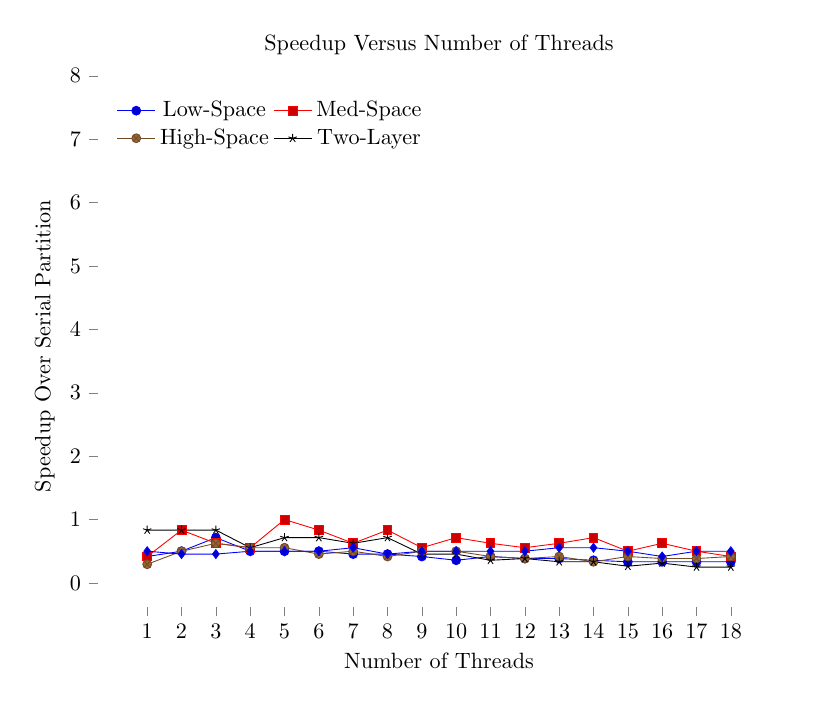
\begin{tikzpicture}[scale = .8]
\begin{axis}[
width = 5 in,
height = 4in,
title={Speedup Versus Number of Threads},
xtick pos=left,
ytick pos=left,
legend style={draw=none},
axis line style = { draw = none },
legend pos= north west,
xtick = data,
xlabel={Number of Threads},
ylabel={Speedup Over Serial Partition},
ymax = 8,
legend columns = 2,
scatter/classes=%
{a={mark=o,draw=blue}}]
%% In-Place
\addplot coordinates {( 1, 0.416667) ( 2, 0.5) ( 3, 0.714286) ( 4, 0.5) ( 5, 0.5) ( 6, 0.5) ( 7, 0.454545) ( 8, 0.454545) ( 9, 0.416667) ( 10, 0.357143) ( 11, 0.416667) ( 12, 0.384615) ( 13, 0.384615) ( 14, 0.357143) ( 15, 0.333333) ( 16, 0.333333) ( 17, 0.333333) ( 18, 0.333333) };
%% In-Place Prefix-Sum
\addplot coordinates {( 1, 0.416667) ( 2, 0.833333) ( 3, 0.625) ( 4, 0.555556) ( 5, 1) ( 6, 0.833333) ( 7, 0.625) ( 8, 0.833333) ( 9, 0.555556) ( 10, 0.714286) ( 11, 0.625) ( 12, 0.555556) ( 13, 0.625) ( 14, 0.714286) ( 15, 0.5) ( 16, 0.625) ( 17, 0.5) ( 18, 0.416667) };
%% Out-of-Place
\addplot coordinates {( 1, 0.294118) ( 2, 0.5) ( 3, 0.625) ( 4, 0.555556) ( 5, 0.555556) ( 6, 0.454545) ( 7, 0.5) ( 8, 0.416667) ( 9, 0.5) ( 10, 0.5) ( 11, 0.416667) ( 12, 0.384615) ( 13, 0.416667) ( 14, 0.333333) ( 15, 0.416667) ( 16, 0.384615) ( 17, 0.384615) ( 18, 0.416667) };
%% High-Span
\addplot coordinates {( 1, 0.833333) ( 2, 0.833333) ( 3, 0.833333) ( 4, 0.555556) ( 5, 0.714286) ( 6, 0.714286) ( 7, 0.625) ( 8, 0.714286) ( 9, 0.454545) ( 10, 0.454545) ( 11, 0.357143) ( 12, 0.384615) ( 13, 0.333333) ( 14, 0.333333) ( 15, 0.263158) ( 16, 0.3125) ( 17, 0.25) ( 18, 0.25) };
%% Cache-Friendly
\addplot coordinates {( 1, 0.5) ( 2, 0.454545) ( 3, 0.454545) ( 4, 0.5) ( 5, 0.5) ( 6, 0.5) ( 7, 0.555556) ( 8, 0.454545) ( 9, 0.5) ( 10, 0.5) ( 11, 0.5) ( 12, 0.5) ( 13, 0.555556) ( 14, 0.555556) ( 15, 0.5) ( 16, 0.416667) ( 17, 0.5) ( 18, 0.5) };
\legend{Low-Space, Med-Space, High-Space, Two-Layer}
\end{axis}
\end{tikzpicture}
}
\def \cilktwoblocksizetwo {64}
\def \cilktwonumtrialstwo {5}
\def \cilktwonumcorestwo {18}
\def \cilktwoinputsizetwo {262144}
\def \cilktwotabletwo {
\begin{tikzpicture}[scale = .8]
\begin{axis}[
width = 5 in,
height = 4in,
title={Speedup Versus Input Size},
xtick pos=left,
ytick pos=left,
legend style={draw=none},
axis line style = { draw = none },
legend pos= north west,
xtick = data,
xlabel={Log Input Size},
ylabel={Speedup Over Serial Partition},
ymax = 5,
ymin = 0,
legend columns = 2,
scatter/classes=%
{a={mark=o,draw=blue}}]
%% Serial Baseline
%% baselines in ms: \addplot coordinates {};
%% In-Place
\addplot coordinates {};
%% In-Place Prefix-Sum
\addplot coordinates {};
%% Out-of-Place
\addplot coordinates {};
%% High-Span
\addplot coordinates {};
%% Cache-Friendly
\addplot coordinates {};
\legend{Low-Space, Med-Space, High-Space, Two-Layer}
\end{axis}
\end{tikzpicture}
}
\def \CILKsortblocksize {64}
\def \CILKsortnumtrials {5}
\def \CILKsortmaxinputsize {262144}
\def \CILKsorttable {
\begin{tikzpicture}[scale = .8]
\begin{axis}[
width = 5 in,
height = 4in,
title={Speedup Versus Number of Threads},
xtick pos=left,
ytick pos=left,
legend style={draw=none},
axis line style = { draw = none },
legend pos= north west,
xtick = data,
xlabel={Number of Threads},
ylabel={Speedup Over Serial Partition},
ymax = 6,
legend columns = 2,
scatter/classes=%
{a={mark=o,draw=blue}}]
\legend{ Low-Space 24, Low-Space 26, Low-Space 28, Two-Layer 24, Two-Layer 26, Two-Layer 28}
\end{axis}
\end{tikzpicture}
}
\def \partitionbandwidthboundserialbaseline {1.4}
\def \partitionbandwidthboundblocksize {64}
\def \partitionbandwidthboundnumtrials {5}
\def \partitionbandwidthboundinputsize {262144}
\def \partitionbandwidthboundtable {
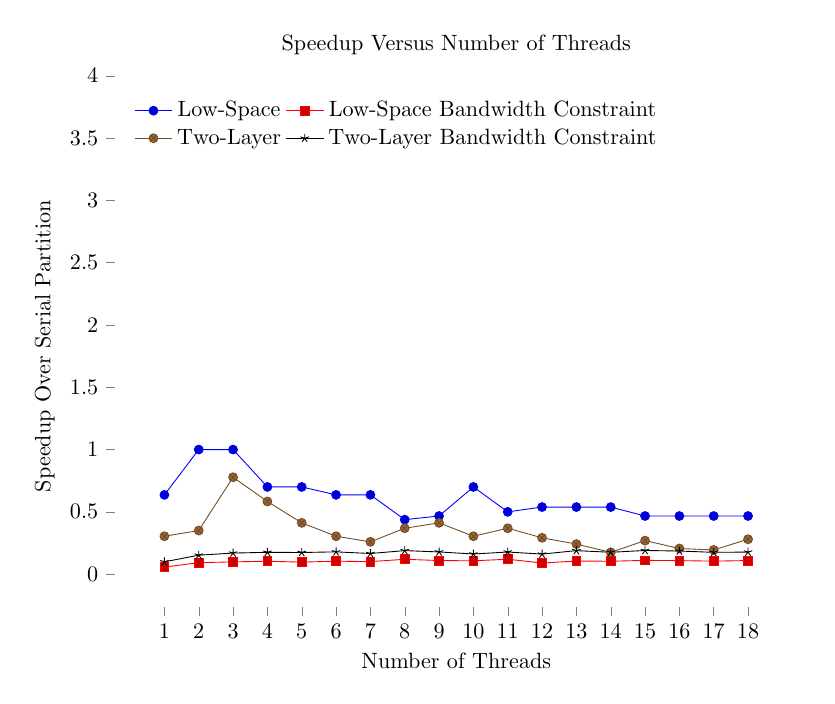
\begin{tikzpicture}[scale = .8]
\begin{axis}[
width = 5 in,
height = 4in,
title={Speedup Versus Number of Threads},
xtick pos=left,
ytick pos=left,
legend style={draw=none},
axis line style = { draw = none },
legend pos= north west,
xtick = data,
xlabel={Number of Threads},
ylabel={Speedup Over Serial Partition},
ymax = 4,
legend columns = 2,
scatter/classes=%
{a={mark=o,draw=blue}}]
%% In-Place
\addplot coordinates {( 1, 0.636364) ( 2, 1) ( 3, 1) ( 4, 0.7) ( 5, 0.7) ( 6, 0.636364) ( 7, 0.636364) ( 8, 0.4375) ( 9, 0.466667) ( 10, 0.7) ( 11, 0.5) ( 12, 0.538462) ( 13, 0.538462) ( 14, 0.538462) ( 15, 0.466667) ( 16, 0.466667) ( 17, 0.466667) ( 18, 0.466667) };
%% Low-Space Bandwidth Bound
\addplot coordinates {(1, 0.0566392)(2, 0.0918376)(3, 0.0985994)(4, 0.103927)(5, 0.0965002)(6, 0.103986)(7, 0.100812)(8, 0.119203)(9, 0.109285)(10, 0.106923)(11, 0.119862)(12, 0.0891909)(13, 0.105142)(14, 0.103583)(15, 0.110553)(16, 0.108612)(17, 0.104464)(18, 0.109112)};
%% high span
\addplot coordinates {( 1, 0.304348) ( 2, 0.35) ( 3, 0.777778) ( 4, 0.583333) ( 5, 0.411765) ( 6, 0.304348) ( 7, 0.259259) ( 8, 0.368421) ( 9, 0.411765) ( 10, 0.304348) ( 11, 0.368421) ( 12, 0.291667) ( 13, 0.241379) ( 14, 0.175) ( 15, 0.269231) ( 16, 0.205882) ( 17, 0.194444) ( 18, 0.28) };
%% High-Span Bandwidth Bound
\addplot coordinates {(1, 0.0989274)(2, 0.152213)(3, 0.16911)(4, 0.175354)(5, 0.173704)(6, 0.178873)(7, 0.165707)(8, 0.188904)(9, 0.178216)(10, 0.161825)(11, 0.177553)(12, 0.161085)(13, 0.188701)(14, 0.175466)(15, 0.190048)(16, 0.185474)(17, 0.175112)(18, 0.176937)};
\legend{Low-Space, Low-Space Bandwidth Constraint, Two-Layer, Two-Layer Bandwidth Constraint}
\end{axis}
\end{tikzpicture}
}
